\chapter{Experimental Design}
\label{ch:dev}
Based on the evaluation of tools and previous work in the area of
steganalysis, an experimental setup is described to test a random sample
of images for steganography. In this section I propose a hypothesis that
is to be tested using the experimental setup. 
\section{Hypothesis}
\label{sec:hypothesis}
In Section \ref{sec:practical}, we discussed the work of Provos and
Honeyman in the area of practical steganalysis. It is proposed to test
the following hypothesis:
\par
\emph{The use of image steganography as a means of covert communication
is non existent as it is possible to reliably identify images containing
data embedded with popular steganographic tools with a reasonably high
degree of accuracy. The primary motive for the use of steganography as a
means of secretive communication in plain sight is effectively nullified
with the availability of detection tools like stegdetect}. 
Additionally, the experiment is subject to the following constraints:
\begin{itemize}
\item{Image Type}: The experiment is focused on analysis JPEG images
gathered from the internet. All other image types are excluded and
ignored by the crawler.
\item{Image Size}: All analysed images are larger than 100x100 pixels in
size and have a colour depth of 24 bits. This threshold has been chosen since it 
is assumed that smaller image sizes would provide very little bandwidth
for steganographic content.
\end{itemize}
\par  Previous experiments that have successfully identified images containing steganographic have done so under lab conditions with strictly defined parameters for image size, colour depth and resolution. Images available online vastly differ in size, resolution and colour depth. Additionally, they might be created using different versions or implementations of the same compression algorithm. 

\section{Control Dataset}
\label{sec:control}
It was required to have a control data set of ``clean'' images to
determine the number of false positives determined by
\texttt{stegdetect} as well as to evaluate the performance of stegdetect. I used a set of personal JPEG images collected from
a Canon S3IS camera over the last few years. The images were scanned
using \texttt{stegdetect} in their original resolution (average 5
Megapixels) as well as after
being cropped to a size of 500x500 pixels.



\section{System Architecture}
\label{sec:sysarch}
\begin{figure}[h!]
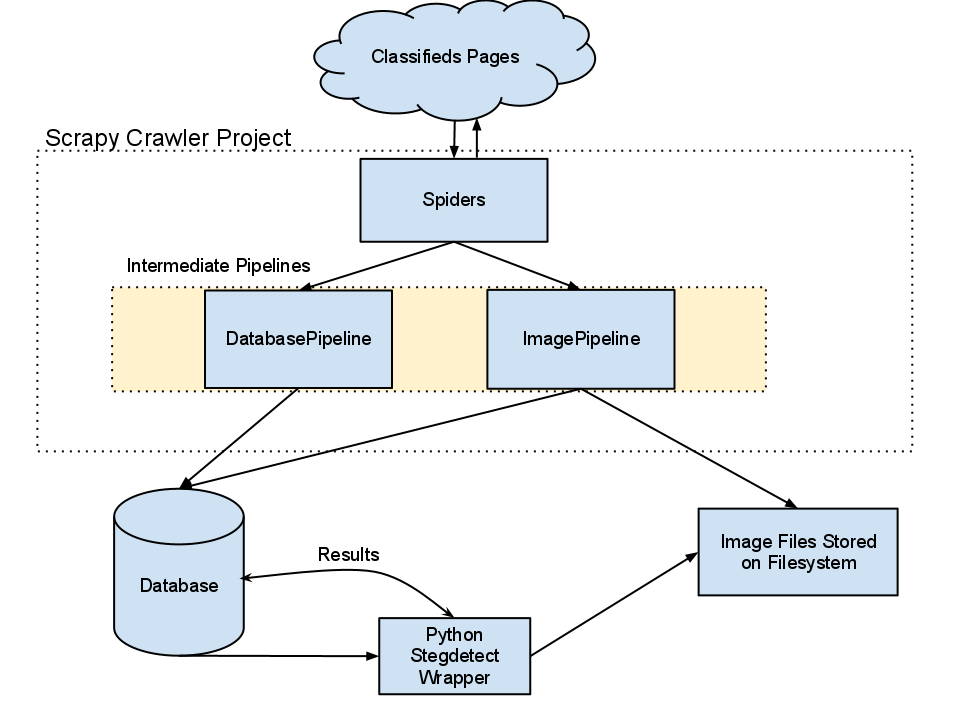
\includegraphics[scale=0.5]{ArchDiagThesis}
\caption{\emph{An overview of the system architecture}}
\label{fig:architecture}
\end{figure} 
\ref{fig:architecture}
%Describe the design
%Describe how all the components fit in together
%Describe how it all differs from the proposal design

\subsection {Web Scraper}
\label{sec:scraper}
%What is a scraper?
%What does it consist of?
%Why do you need it for these project?
%Why did you choose scrapy?
%How does it work?
A scraper allows an application to retrieve and store specific items from a web page. Any part of the HTML Document Object Model (DOM) can be selected and extracted for further processing, a process known as scraping. Most crawlers consist of two main components, a web crawler that allows it to collect a large number of pages quickly and the actual scraping module that allows for the extraction of relevant content. A large number of free and open source projects are available that provide both kinds of functionality. For this project, scrapy was used as the basis for the web scraper based on previous evaluations and it's excellent database connectivity and image handling options.
\par Scrapy is a python web framework that can be used to build web crawlers/scrapers. It was designed primarily for programmatically accessing websites that do not explicitly provide an Application Programming Interface (API). Scrapy does not provide an implementation of a specific scraper, it provides a number of classes that can be used to create a custom scraper. A scrapy project consists of one or more spiders and pipelines that determine what happens once an item has been downloaded. The crawler component was created by extending scrapy's \texttt{BaseSpider} class. The \texttt{BaseSpider} class requires the implementation of a \texttt{parse()} method that determines the action to be taken when an HTML page is encountered. The \texttt{parse()} method is called on every invocation of the spider. Relevant elements in the HTML page are selected using HTML XPath queries. In this implementation, the \texttt{parse()} method yields subsequent HTTP requests that the crawler needs to make subsequently using the URLs found on the page. An \texttt{Item} class is also created for each JPEG image found on the page. These images are then added to a python dictionary and returned to the \texttt{ImagePipeline} middleware.
\par The \texttt{ImagePipeline} middleware is responsible for the scheduling and downloading of image files. For each dictionary of items returned by the crawler, the pipeline enqueues the URLs of the images found and downloads them asynchronously. Saved images are named according to the MD5 hash of their content so that they can be uniquely identified at a later stage. After building a suitably large collection of images, steganalysis was carried out on each of the images as described in the next section.
\subsection {Steganalysis}
\label{sec:stegtool}
Steganalysis on the downloaded images is carried out using \texttt{stegdetect} which is part of Provos' Outguess suite of steganography tools. \texttt{stegdetect} provides detection features for six different kinds of JPEG steganographic algorithms namely jsteg, outguess, jphide, invisible secrets, F5 and text appending. For each steganographic algorithm detected by \texttt{stegdetect} it provides a confidence rating between one to three stars. It also provides a parameter for tuning the sensitivity of the scanner. The sensitivity can be specified as a floating point number, which would cause the confidence rating to be multiplied by it. For this project, \texttt{stegdetect} was used only to try and detect algorithms known to it although stegdetect allows for feature extraction that can be used to detect unknown algorithms. The detection was carried out using four different sensitivity settings (0.25,0.5,0.75 and 1) in order to minimize false positives.
\par A custom python script was created to wrap \texttt{stegdetect} and generate output in a way suitable for database storage. Finally, the data obtained was saved in a database for further analysis.
\subsection{Database Structure}
\label{sec:dbstructure}
The initial database chosen for the project was sqlite as the application had modest data requirements. However, sqlite ended up causing a large amount of data corruption and was the source of thread concurrency errors. The data was then migrated to a MySQL database and the code was modified accordingly.A single data table stores details of the downloaded images which are generated by the middleware after each image has been downloaded. 
\par Each image is uniquely identified in the database by an auto incrementing primary key. Steganalysis is carried out by obtaining the path of each image from the database and running stegdetect on them. The results of the stegnalayis are stored in an analysis table which uniquely identifies each result by an autoincrementing primary key and references the primary key of the image from the data table.
\par  All access to the database is through a connection pool that maintains 4 connections to the MySQL database. This was implemented by extending a class from the python twisted library called the Asynchronous Database Access API (twisted.enterprise.adbapi). Adbapi provides a non blocking interface to the database and vastly improves random read/write access when compared to standard database APIs like the standard python MySQLdb API. The adbapi class was modified to handle reconnections to the database as it was discovered that the provided MySQL database frequently dropped connections between transactions. 
